%%%%%%%%%%%%%%%%%%%%%%%%%%%%%%%%%%%%%%%%%%%%%%%%%%%%%%%%%%%%%%%%%%%%%%%%%%%%%%%%%%%%%%%%%%%%%%%%%%%
\chapter{Introdução}

O contínuo crescimento da população mundial trouxe consigo um massivo aumento da exploração dos recursos naturais do planeta Terra, tais como plantas, animais e minerais. As plantas são usadas pelos seres humanos desde a antiguidade tanto para a alimentação como para o tratamento de diversas doenças. Muitas das espécies que surgem no mundo, numa primeira fase são consideradas pragas. Contudo, e após alguns estudos intensivos, são descobertas verdadeiras preciosidades devido às propriedades que apresentam\cite{Verma2008}\cite{Newman2012}. Um exemplo disso é a planta que servirá de contexto à elaboração desta dissertação, denominada por \sr. Esta é uma planta suculenta adaptada a ambientes aquáticos com elevado teor de sal que cresce ao longo dos estuários e sapais (salinas) costeiros do Mediterrâneo\cite{Ventura2011}. Esta planta é utilizada para os mais diversos fins nomeadamente, como substituto do sal marinho\cite{jnsalic}. 


%\begin{figure}[!htb]
%\centering
%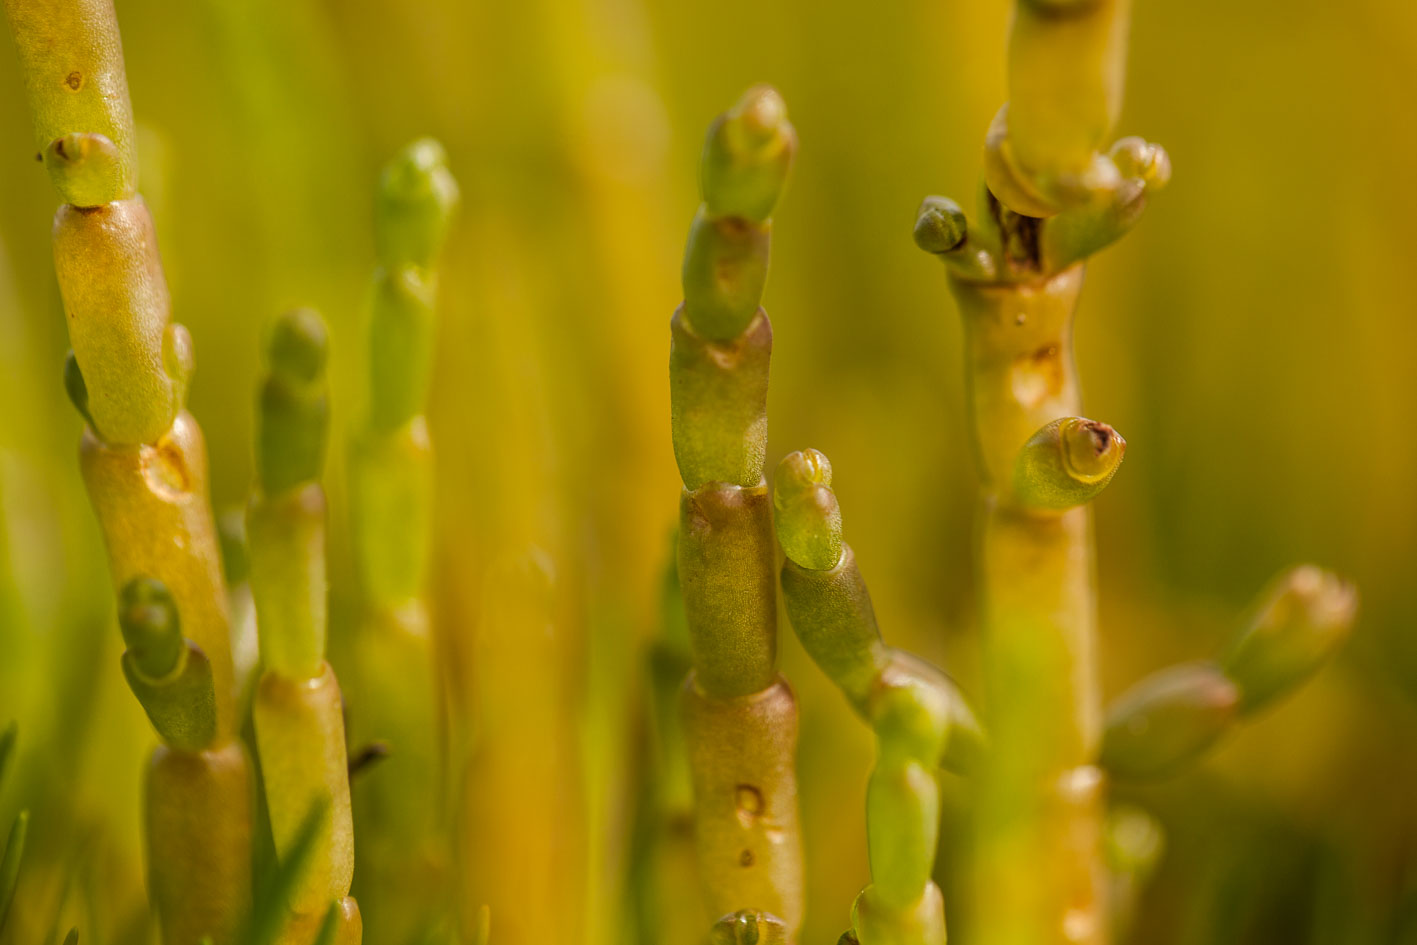
\includegraphics[scale= 0.25]{img/cap2-sali/Salicornia05.JPG}
%\caption{Salicórnia na Ria de Aveiro (Fotografia por José M. G. Pereira)}
%\label{saliintr}
%\end{figure}



Nos dias de hoje, nos processos de agricultura intensiva, há necessidade de otimizar os mecanismos de produção controlando certos aspetos ambientais para obter o maior proveito dos recursos e, ao mesmo tempo, a garantia da qualidade dos produtos. Assim, torna-se fulcral conhecer as condições ideais para o melhor crescimento da espécie. Para entender quais os fatores que influenciam esse desenvolvimento, é necessária a existência de equipamentos sensoriais que recolham e transmitam os dados obtidos, a fim de serem analisados e processados. Por outro lado, é essencial garantir que esses parâmetros se encontram dentro dos valores ótimos através de mecanismos inteligentes capazes de atuar e desencadear processos de correção ao sistema sempre que o ambiente está fora desses parâmetros. 


Uma vez que o cultivo da Salicórnia é relativamente recente, existe um grande interesse, por parte dos biólogos e dos agricultores, em entender de que forma certos parâmetros podem influenciar o crescimento da espécie, com a intenção de otimizar a produtividade e rentabilidade do seu cultivo. Com este propósito e tirando partido da evolução tecnológica, pretende-se desenvolver um sistema que permita a introdução da sensorização no cultivo da Salicórnia.     


\section{Motivação}

O incentivo desta dissertação consiste em incluir sensorização na produção de Salicórnia, com o propósito de, através da consecutiva monitorização, oferecer dados reais para que os investigadores do Departamento de Biologia da Universidade de Aveiro possam identificar as condições ideais de certos parâmetros favoráveis ao seu crescimento. Adicionalmente, esta solução servirá de embrião para um sistema de controlo e monitorização idealizado por uma empresa da região de Aveiro que se dedica à produção de Salicórnia, denominada por ``Horta dos Peixinhos"\footnote{\url{http://hortadospeixinhos.com/}}. Este sistema permitirá agilizar o mecanismo de transferência de águas, automatizando todo o processo de irrigação e cultivo desta espécie. 



%O quatro do cultivo de Salicórnia apresentado pela empresa indica outros desafios, como a ausência de locais de fornecimento de energia 


%O cenário de cultivo de salicórnia representa outros desafios, como a inexistência de locais de fornecimento de energia ou infraestruturas de comunicação com fios. Estas  caraterísticas, aliadas ao facto de estes sensores servirem apenas para a aquisição e transmissão de informação pouco frequente e de baixo volume, tornam este cenário claramente num cenário que encaixa no universo da Internet Of Things (IoT).

\section{Objetivos}
\label{objectivos}

O objetivo geral desta dissertação é desenvolver um sistema de informação que permita monitorizar e controlar o cultivo da Salicórnia. Para tal, pretende-se criar um protótipo em \textit{hardware} que permita  simular o cenário desejado. Idealiza-se que a solução encontrada esteja inserida no universo do \ac{IoT}\cite{Farooq2015}, tanto quanto possível, isto é, que apresente alguma escalabilidade, baixo custo, autonomia total de funcionamento e capacidade de comunicação sem fios. Face aos objetivos supracitados, estabeleceram-se os seguintes objetivos específicos:

\begin{enumerate}

	\item Recolher os requisitos do cliente e definir as funcionalidades com base na respetiva modelação; 
	
	\item Definir uma arquitetura para o cenário apresentado, tornando-o apto a ser adaptado a outros contextos; 
	
	\item Desenvolver uma \ac{API} que disponibilize os serviços deste sistema, possibilitando a criação de novas aplicações;   
	
	\item Criar uma plataforma \textit{web} que permita a  interação simples e intuitiva com o utilizador para disponibilizar a leitura de dados dos diferentes sensores; 
	
	\item Permitir que o utilizador do sistema atue remotamente na ativação/desativação de atuadores; 
	
	
	\item Gerar alarmes quando os valores obtidos pelos sensores estão fora da gama dos valores ideais; 
	
	\item Simular em \textit{hardware} o cenário apresentado, utilizando alguns sensores ambientais e comunicação sem fios; 
	
	\item Criar um sistema de videovigilância que permita a deteção de intrusos e supervisionar os campos de cultivo. 

\end{enumerate}

%2) Definição das funcionalidades da plataforma e dos alarmes; 3) Implementação de um protótipo de plataforma; 4) Desenvolvimento das Apps para comunicação com a plataforma e com o terreno;

\section{Metodologia de trabalho}
\label{method}


Para a elaboração do trabalho prático desta dissertação, foi adotada uma metodologia de investigação orientada à engenharia\cite{desingprocess}. Esta metodologia, assenta num conjunto de passos continuados pelos engenheiros que permitem encontrar um conjunto de soluções para dar resposta aos problemas em questão. Os principais passos, centram-se sobretudo na definição dos problemas e investigação do tema, especificação dos requisitos, \textit{brainstorm} de soluções e escolha da melhor, desenvolvimento do trabalho, criação de protótipos e respetivos testes da solução. Por fim, se a solução não for de encontro com os requisitos estabelecidos, o processo é realizado novamente\cite{desingprocess}. Este modelo é conhecido como metodologia de desenvolvimento iterativo e incremental. 


\begin{figure}[!htb]
	\centering
	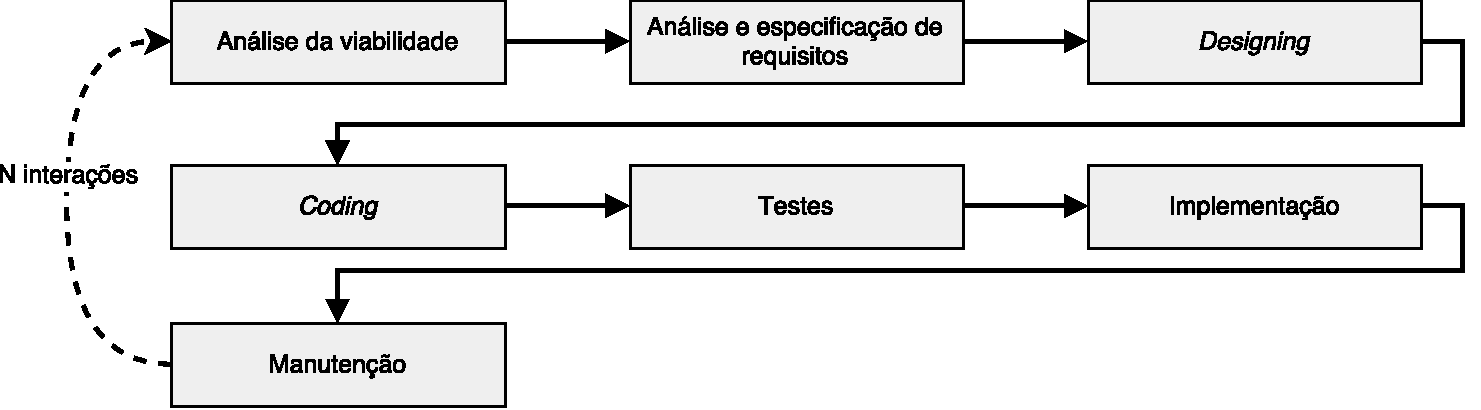
\includegraphics[scale=0.6]{esquemas/desenvolvimentoSW.pdf}
	\caption[Fases de desenvolvimento de um \textit{software} ]{Fases de desenvolvimento de um \textit{software} (Adaptado de \cite{Saini2014})}
	\label{sdlcartic}
\end{figure}


No contexto do desenvolvimento da solução desta dissertação, foram consideradas várias etapas do ciclo de vida de desenvolvimento de um \textit{software} definidas por  \textit{Saini e Kaur}\cite{Saini2014}. Este, também conhecido como \ac{SDLC}, é composto genericamente por quatro fases principais: conceção, projeção, criação e implementação. Antes do \ac{SDLC}, o processo de desenvolvimento de \textit{software} era tomado como uma atividade informal sem regras nem padrões. Isto pode dar  origem a vários problemas, tais como o atraso no desenvolvimento, aumento dos custos e baixa qualidade do \textit{software} criado. Existem inúmeros modelos e visões que propõem alguns padrões e etapas necessárias ao desenvolvimento de um sistema com qualidade. Na figura \ref{sdlcartic} encontram-se as sete etapas consideradas por \textit{Saini e Kaur}\cite{Saini2014} que seguidamente serão descritas. 

\begin{itemize}
	\item \textbf{Análise da viabilidade}: nesta fase são analisados os dados de entrada e saída, processamento necessário, análise de custos e planeamento do projeto. É ainda incluída a viabilidade técnica em termos de \textit{software}, \textit{hardware} e pessoas qualificadas;
	
	\item \textbf{Análise e especificação de requisitos}: nesta fase são recolhidos e analisados os requisitos necessários para a elaboração do \textit{software}. No final, pretende-se que sejam conhecidos os vários requisitos do \textit{software} e seja também criado um documento que os especifique; 
	
	\item  \textbf{Desenho/Concepção} (\textit{Designing}): consiste na tradução dos requisitos especificados para uma estrutura lógica. No final, prevê-se que seja elaborado um documento de especificação do \textit{design}; 
	
	
	\item  \textbf{Programação} (\textit{Coding}): a programação real é elaborada nesta fase. O documento de \textit{design} é traduzido para o código-fonte numa determinada linguagem de forma a que possa ser executado;
	
	\item \textbf{Testes}: o código-fonte gerado na fase anterior é testado usando vários cenários de teste com o objetivo de corrigir e avaliar o \textit{software}; 
	
	\item  \textbf{Implementação}: o \textit{software} desenvolvido é implementado para que possa ser disponibilizado ao utilizador para uso real. Pretende-se que o utilizador do sistema possa reportar erros ou problemas quando encontrados; 
	
	\item  \textbf{Manutenção}: o \textit{software} poderá sofrer alterações para solucionar problemas que possam ter sido encontrados. Esta fase é responsável pela pós-implementação e manutenção do \textit{software} para o seu bom funcionamento.
	
\end{itemize}


Adicionalmente, durante o desenvolvimento do trabalho prático desta dissertação foram criados alguns repositórios Git\footnote{\url{https://git-scm.com/}} que permitiram controlar as diferentes versões do código desenvolvido, permitindo ainda um \textit{backup} sistemático e um armazenamento seguro. No contexto deste trabalho, a existência de um sistema de controlo de versões foi especialmente importante já que permitiu recuperar versões anteriores. 


\section{Organização do documento}


A presente dissertação encontra-se dividida em sete capítulos. No primeiro capítulo, \textbf{Introdução}, é descrita e enfatizada a importância da monitorização e controlo do cultivo da Salicórnia, bem como os principais objetivos desta dissertação. Seguidamente, no capítulo dois, \textbf{O \ac{IoT} no cultivo da Salicórnia}, será apresentada a Salicórnia destacando as suas características e importância. Para além disso, será  
exposta a evolução tecnológica até ao universo do \ac{IoT}. De seguida, o capítulo três, \textbf{Estado da arte}, contém o enquadramento teórico onde são abordadas as tecnologias possíveis de utilização bem como a respetiva comparação. No quarto capítulo, \textbf{Sistema de controlo e monitorização: arquitetura e modelação}, são apresentados todos os requisitos do sistema, realizada a modelação do mesmo e apresentada a sua arquitetura. Posteriormente, no quinto capítulo, \textbf{Implementação}, é descrita a conceção e implementação do sistema e dos seus vários componentes. No sexto capítulo,\textbf{ Testes e resultados}, são apresentados alguns testes funcionais e respetivos resultados do sistema desenvolvido. Finalmente, no sétimo capítulo, \textbf{Conclusão e trabalho futuro}, é analisado e refletido todo o trabalho realizado nesta dissertação por forma a concluir se os resultados obtidos satisfazem os objetivos previamente definidos. No fim, será mencionado e discutido todo o trabalho futuro que possa vir a ser realizador com intenção de aperfeiçoar a solução proposta. 

%O primeiro capítulo descreve e enfatiza a importânci

%De seguida, no Estado de Arte, é


%No Capítulo 2 apresenta-se 

%o projeto CAMBADA e identifica-se os pontos chave tanto do software como do hardware. No Capítulo 3 

%No Capítulo 4 é.... 

%Para finalizar, no Capıtulo 5 apresentam-se conclusões sobre o trabalho desenvolvido e eventuais melhorias para o futuro.

%Resumo As elevadas propriedades nutricionais da \textit{Salicornia L.} tornam-na atrativa para aplicações culinárias e para o tratamento e prevenção de algumas doenças.






